% Chapter Template
\chapter{Trabajo Realizado} % Main chapter title

\label{Chapter2} % Change X to a consecutive number; for referencing this chapter elsewhere, use \ref{ChapterX}

%----------------------------------------------------------------------------------------
%	SECTION 1
%----------------------------------------------------------------------------------------
Esto probablemente tendrá muchas secciones y subsecciones que ire agregando conforme vaya haciendo cosas. Por lo pronto lo unico que tengo para poner aca es que hice una red de 4 ruters con libremesh y anda. Ponerle algunas screenshots y una foto pochoclera como la de la figura (\ref{RedMeshCasera1}).

\begin{figure}[th]	
	\centering	
	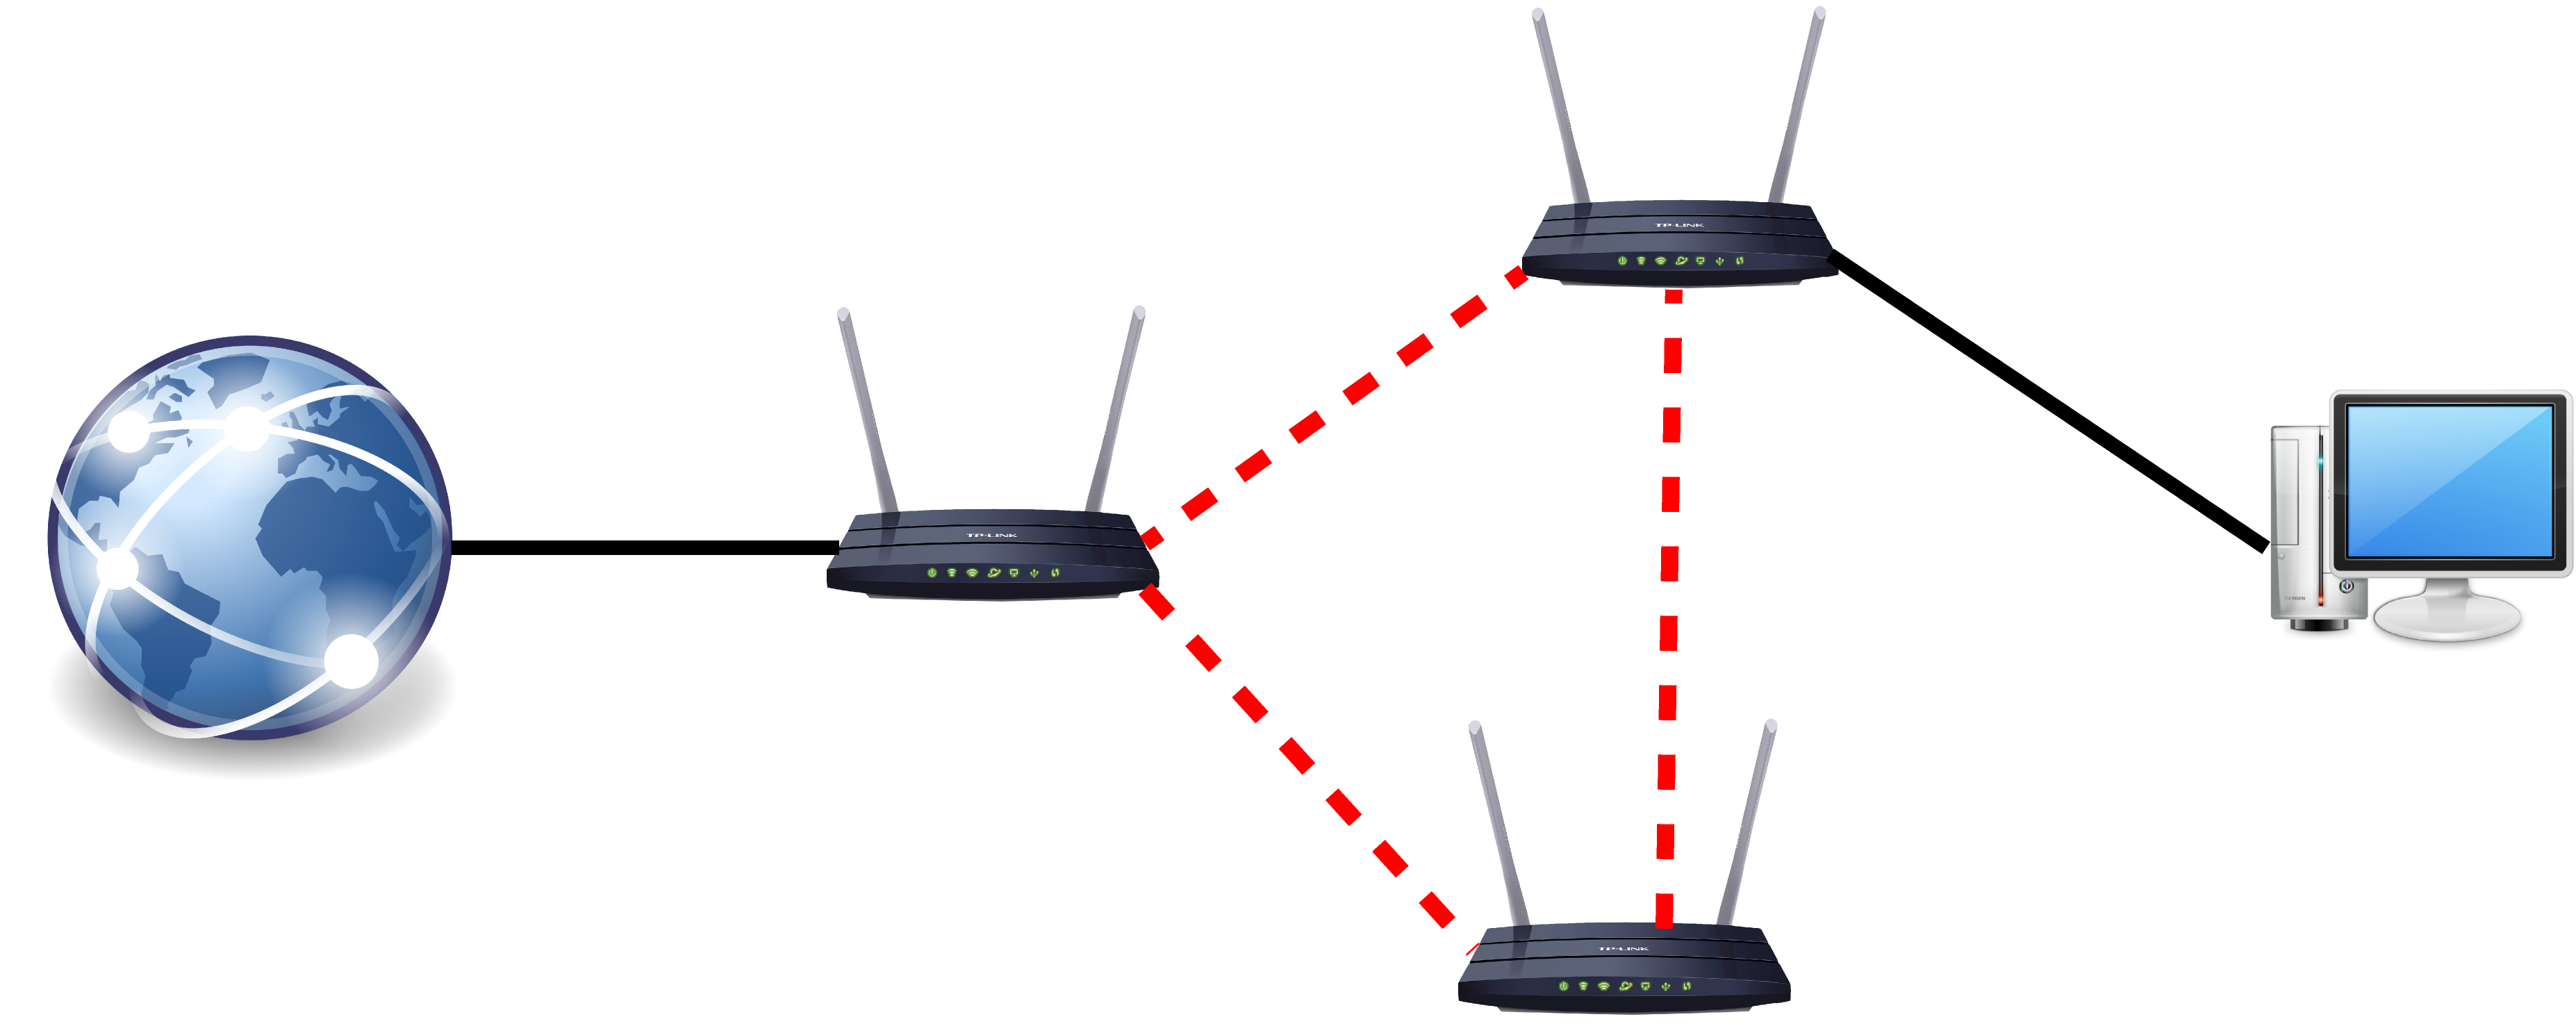
\includegraphics[width=0.7\textwidth]{./figures/RedMeshCasera1.png}		
	\caption{\textit{Topología de primer red mesh realizada.}}
	\label{RedMeshCasera1}
\end{figure}






